\chapter{Literature Review}\label{ch:literature}

This chapter provides a comprehensive review of the theoretical foundations, prior electronic voting systems, blockchain-based voting proposals, and anonymous credential schemes that inform the design of our privacy-preserving voting system. We identify critical gaps in the existing literature and position our contribution within the broader landscape of cryptographic voting research.

\section{Theoretical Foundations}

\subsection{Zero-Knowledge Proofs}

A zero-knowledge proof (ZKP) is an interactive or non-interactive protocol between a prover $\mathcal{P}$ and a verifier $\mathcal{V}$ that enables $\mathcal{P}$ to convince $\mathcal{V}$ that a statement $x$ is true without revealing any information beyond the truth of the statement~\cite{goldwasser1989knowledge}.

\begin{definition}[Zero-Knowledge Proof System]
A proof system $(P, V)$ for a language $L$ is zero-knowledge if it satisfies:
\begin{enumerate}
    \item \textbf{Completeness}: If $x \in L$, then $\Pr[V \text{ accepts}] \geq 1 - \text{negl}(\lambda)$.
    \item \textbf{Soundness}: If $x \notin L$, then $\Pr[V \text{ accepts}] \leq \text{negl}(\lambda)$.
    \item \textbf{Zero-Knowledge}: $\exists$ simulator $S$ such that $\text{View}_V(P, V, x) \approx S(x)$.
\end{enumerate}
\end{definition}

The evolution from interactive to non-interactive zero-knowledge proofs (NIZKs) was enabled by the Fiat--Shamir heuristic~\cite{fiat1986prove}, which replaces the verifier's random challenges with hash function outputs. This transformation is critical for blockchain applications where the prover and verifier cannot interact in real-time.

\begin{equation}
\text{Fiat-Shamir}: \quad c = H(\text{transcript} \| \text{commitment})
\label{eq:fiat-shamir}
\end{equation}

\subsubsection{zk-SNARK Evolution}

The field of succinct non-interactive arguments of knowledge (zk-SNARKs) has evolved rapidly since Groth's seminal 2016 construction~\cite{groth2016size}:

\begin{table}[H]
\centering
\caption{Evolution of ZK proof systems relevant to voting applications.}
\label{tab:zk-evolution}
\begin{tabular}{|l|l|l|l|l|}
\hline
\textbf{System} & \textbf{Year} & \textbf{Trusted Setup} & \textbf{Proof Size} & \textbf{Verify Time} \\
\hline
Groth16 & 2016 & Per-circuit & 128 B & 1.5 ms \\
\hline
PLONK & 2019 & Universal (SRS) & 384 B & 5 ms \\
\hline
Halo2 & 2020 & None (IPA) & 5--10 KB & 200 ms \\
\hline
UltraHonk & 2023 & None (Keccak) & 2--4 KB & $<5$ ms \\
\hline
\end{tabular}
\end{table}

UltraHonk, developed by Aztec Labs as part of the Barretenberg library, represents the state-of-the-art for client-side proving. Its elimination of the trusted setup requirement makes it particularly suitable for voting systems where ceremony coordination presents logistical challenges~\cite{aztec2023ultrahonk}.

\begin{figure}[H]
\centering
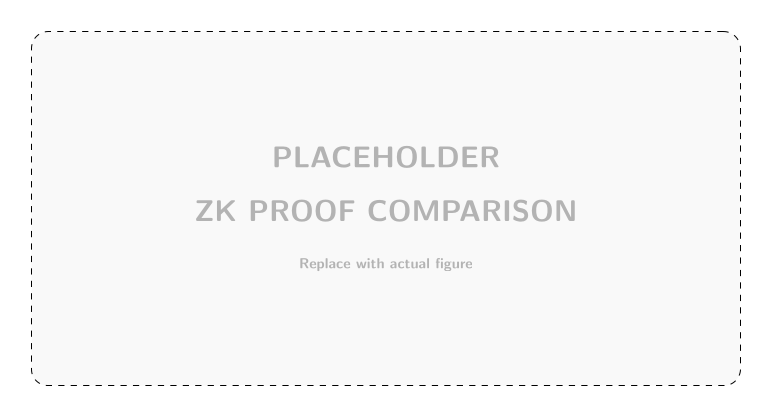
\includegraphics[width=0.85\textwidth]{Images/fig_zk_proof_comparison.png}
\caption{Comparative analysis of ZK proof systems across key dimensions: proof size, verification cost, setup requirements, and prover complexity.}
\label{fig:zk-comparison}
\end{figure}

\subsection{Poseidon Hash Function}

The Poseidon hash function~\cite{grassi2021poseidon} was specifically designed for arithmetic circuits over prime fields, making it orders of magnitude more efficient than algebraically-unfriendly hash functions like SHA-256 or Keccak when expressed as R1CS or Plonkish constraints.

\begin{definition}[Poseidon Permutation]
For a state width $t$ over a prime field $\mathbb{F}_p$, the Poseidon permutation $\pi: \mathbb{F}_p^t \to \mathbb{F}_p^t$ consists of:
\begin{enumerate}
    \item $R_f$ full rounds: $\text{ARK} \to \text{S-box}^t \to \text{MDS}$
    \item $R_p$ partial rounds: $\text{ARK} \to \text{S-box}^1 \to \text{MDS}$
    \item $R_f$ full rounds: $\text{ARK} \to \text{S-box}^t \to \text{MDS}$
\end{enumerate}
where the S-box is $x \mapsto x^\alpha$ with $\alpha = 5$ for BN254.
\end{definition}

The constraint cost comparison is dramatic:

\begin{table}[H]
\centering
\caption{Hash function constraint costs in BN254 arithmetic circuits.}
\label{tab:hash-constraints}
\begin{tabular}{|l|r|r|l|}
\hline
\textbf{Hash Function} & \textbf{Constraints} & \textbf{Ratio} & \textbf{Native to BN254?} \\
\hline
SHA-256 & $\sim$25,000 & 83$\times$ & No (bitwise) \\
\hline
Keccak-256 & $\sim$150,000 & 500$\times$ & No (bitwise) \\
\hline
MiMC & $\sim$730 & 2.4$\times$ & Yes \\
\hline
Poseidon ($t=3$) & $\sim$300 & 1$\times$ & Yes \\
\hline
\end{tabular}
\end{table}

For our system, we use two Poseidon variants:
\begin{align}
\Poseidon_1(x) &: \mathbb{F}_p \to \mathbb{F}_p \quad \text{(nullifier hash)} \\
\Poseidon_2(x, y) &: \mathbb{F}_p^2 \to \mathbb{F}_p \quad \text{(commitment, Merkle nodes)}
\end{align}

\subsection{Merkle Trees for Set Membership}

A Merkle tree~\cite{merkle1987digital} provides $O(\log n)$ proofs of set membership. Given a set of $n$ leaves $\{l_0, l_1, \ldots, l_{n-1}\}$, any leaf can prove membership by revealing only $\log_2 n$ sibling hashes along its authentication path.

\begin{equation}
\text{root} = H\left(H\left(H(l_0, l_1), H(l_2, l_3)\right), H\left(H(l_4, l_5), H(l_6, l_7)\right)\right)
\label{eq:merkle-root}
\end{equation}

The Lean Incremental Merkle Tree (LeanIMT)~\cite{semaphore2023lean} optimizes on-chain storage by only storing nodes along the ``frontier''---the rightmost path---reducing storage from $O(n)$ to $O(\log n)$ while maintaining the same root computation.

\begin{figure}[H]
\centering
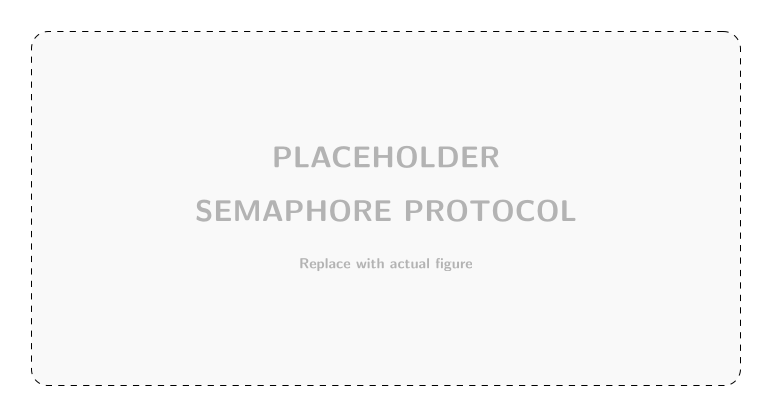
\includegraphics[width=0.85\textwidth]{Images/fig_semaphore_protocol.png}
\caption{Merkle tree membership proof: the prover reveals the path siblings (shaded) but not which leaf is theirs.}
\label{fig:merkle-membership}
\end{figure}

\subsection{BN254 Elliptic Curve}

The BN254 curve (also known as alt\_bn128 or bn256) is a Barreto--Naehrig pairing-friendly elliptic curve defined over a 254-bit prime field~\cite{barreto2005pairing}:

\begin{equation}
E: y^2 = x^3 + 3 \quad \text{over } \mathbb{F}_p
\end{equation}

where $p = 21888242871839275222246405745257275088696311157297823662689037894645226208583$.

The scalar field order (the field in which our circuit operates) is:
\begin{equation}
r = 21888242871839275222246405745257275088548364400416034343698204186575808495617
\end{equation}

BN254 is natively supported by the Ethereum Virtual Machine through precompiled contracts at addresses \texttt{0x06} (addition), \texttt{0x07} (scalar multiplication), and \texttt{0x08} (pairing check)~\cite{eip196,eip197}. This hardware-level support enables gas-efficient on-chain proof verification---a critical requirement for blockchain voting systems.

\section{Electronic Voting Systems: A Historical Perspective}

\subsection{First-Generation Systems (2005--2015)}

\begin{figure}[H]
\centering
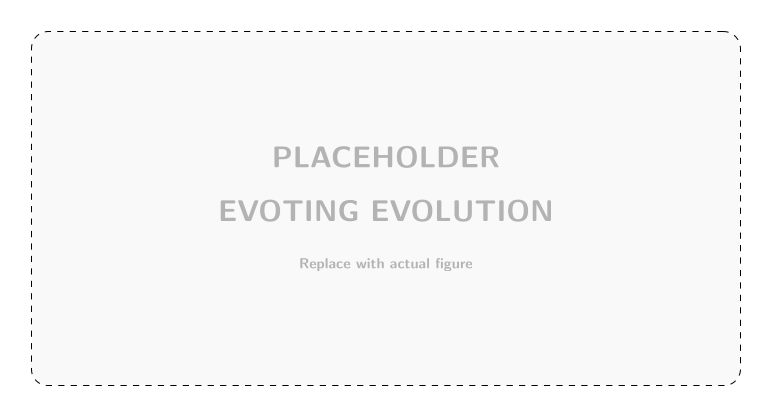
\includegraphics[width=0.85\textwidth]{Images/fig_evoting_evolution.png}
\caption{Evolution of electronic voting systems from centralized servers to blockchain-based privacy-preserving architectures.}
\label{fig:evoting-evolution}
\end{figure}

\subsubsection{Estonia's i-Voting (2005--Present)}

Estonia launched the world's first legally binding internet voting system in 2005~\cite{heiberg2012internet}. The system uses a double-envelope scheme:
\begin{enumerate}
    \item The voter signs their ballot with their national ID card (RSA-2048).
    \item A server strips the identity layer before tallying.
    \item Re-voting is permitted (last vote counts) as coercion mitigation.
\end{enumerate}

\textbf{Strengths}: Government-backed PKI, high adoption (51.1\% in 2023 elections), re-voting for coercion resistance.

\textbf{Weaknesses}: Server-side decryption creates a single point of failure~\cite{springall2014security}. An adversary with access to the collection server can deanonymize all votes. The system assumes trust in the election authority---precisely the assumption we aim to eliminate.

\subsubsection{iVote (New South Wales, Australia)}

The iVote system, deployed for state elections from 2011 to 2021, used a mix-net approach for anonymization~\cite{culnane2015verivote}. Voters authenticated via a PIN mailed to their registered address, then cast votes through a web interface. The system was retired after security researchers demonstrated that a TLS man-in-the-middle attack could modify votes in transit~\cite{halderman2015internet}.

\subsubsection{Swiss Post E-Voting}

Switzerland's Scytl-built system employed verifiable shuffles~\cite{haenni2017swiss} with individual verifiability codes. In 2019, a critical vulnerability was discovered in the decryption shuffle proof that could allow undetected vote manipulation~\cite{lewis2019swiss}. The system was suspended pending redesign.

\subsection{Second-Generation: Cryptographically Verifiable Systems}

\subsubsection{Helios (2008)}

Helios~\cite{adida2008helios} represents a landmark in verifiable voting. It uses ElGamal encryption with a mix-net for anonymization:

\begin{enumerate}
    \item Voter encrypts ballot: $c = \text{Enc}_{pk}(\text{vote}; r)$
    \item Encrypted ballot posted to public bulletin board
    \item Mix-net shuffles and re-encrypts
    \item Threshold decryption reveals tallied results
\end{enumerate}

\begin{figure}[H]
\centering
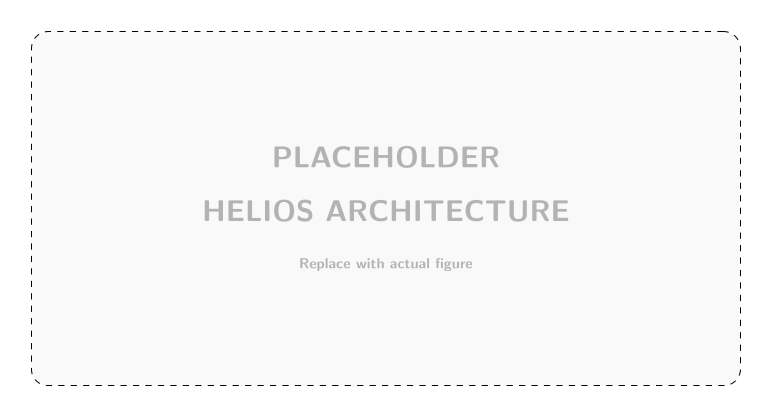
\includegraphics[width=0.85\textwidth]{Images/fig_helios_architecture.png}
\caption{Helios architecture: encrypted ballots are posted publicly, shuffled through a mix-net, and tallied via threshold decryption.}
\label{fig:helios-arch}
\end{figure}

\textbf{Limitations for our context}:
\begin{itemize}
    \item Requires trusted mix-net servers (at least one must be honest)
    \item No coercion resistance (voter can prove their vote via the ballot tracker)
    \item Not designed for blockchain integration
    \item Scalability issues with large electorates (16M+ voters)
\end{itemize}

\subsubsection{Belenios (2017)}

Belenios~\cite{cortier2017belenios} extended Helios with stronger verifiability properties but inherited the mix-net dependency. It introduced a credential-based approach where voters receive a private credential from a registrar, preventing ballot stuffing even if the voting server is compromised.

\subsection{Third-Generation: Blockchain-Based Voting}

\subsubsection{Voatz (2018--2020)}

Voatz deployed mobile blockchain voting in West Virginia (2018), Denver (2019), and several other jurisdictions for absentee military voters~\cite{voatz2020}. The system used a permissioned Hyperledger-based blockchain with biometric authentication.

\begin{figure}[H]
\centering
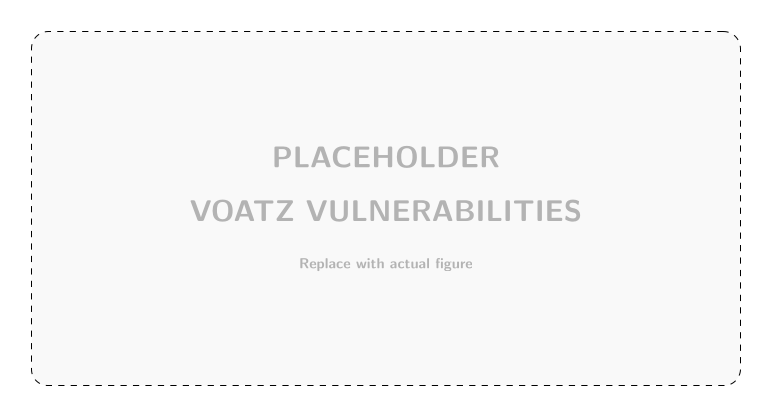
\includegraphics[width=0.85\textwidth]{Images/fig_voatz_vulnerabilities.png}
\caption{Security vulnerabilities identified in the Voatz system by MIT researchers, including the lack of end-to-end verifiability.}
\label{fig:voatz-vuln}
\end{figure}

In 2020, MIT researchers~\cite{specter2020ballot} identified critical vulnerabilities:
\begin{itemize}
    \item Server-side sees plaintext votes (no encryption)
    \item Biometric data transmitted to central server
    \item No end-to-end verifiability
    \item Client-side code obfuscated (prevents audit)
    \item Blockchain used only as append-only log (no cryptographic voting properties)
\end{itemize}

The Voatz case demonstrates that blockchain alone provides no ballot privacy---it merely records transactions transparently, making the privacy problem \textit{worse} unless cryptographic measures are added.

\subsubsection{McCorry et al. --- Open Vote Network (2017)}

McCorry, Shahandashti, and Hao~\cite{mccorry2017smart} proposed the first decentralized voting protocol on Ethereum. Their ``Open Vote Network'' uses a two-round protocol:
\begin{enumerate}
    \item Each voter publishes a public key $g^{x_i}$
    \item Each voter publishes $g^{x_i \cdot Y_i} \cdot g^{v_i}$ where $Y_i$ is derived from other keys
    \item The tally is computed from the product of all ciphertexts
\end{enumerate}

\textbf{Limitations}: Only supports yes/no votes, $O(n)$ on-chain gas cost per voter, no support for multi-candidate elections, limited to $\sim$50 voters due to gas constraints.

\subsubsection{Agora (2017)}

Agora~\cite{agora2017} attempted blockchain voting in Sierra Leone's 2018 elections (observer capacity only). Their approach used a permissioned chain with a ``Skipchain'' structure. However, the system lacked formal privacy guarantees and relied on physical presence verification with no cryptographic anonymization.

\subsection{Fourth-Generation: ZK-Based Blockchain Voting}

\subsubsection{MACI --- Minimum Anti-Collusion Infrastructure (2020)}

MACI~\cite{buterin2020maci}, proposed by Vitalik Buterin and implemented by the Privacy \& Scaling Explorations team at the Ethereum Foundation, addresses the collusion/bribery problem:

\begin{enumerate}
    \item Voters encrypt their votes with a coordinator's public key
    \item The coordinator processes encrypted votes in a zk-SNARK circuit
    \item Vote changes (re-voting) are hidden from observers
    \item The coordinator publishes a proof that the tally is correct
\end{enumerate}

\textbf{Key Innovation}: MACI allows voters to change their vote secretly, making bribery unenforceable---even if a voter shows a briber their initial vote, they can later override it without detection.

\textbf{Limitations}:
\begin{itemize}
    \item \textbf{Coordinator dependency}: A single coordinator processes all votes. If compromised, ballot privacy is lost (though integrity is maintained by the ZK proof).
    \item \textbf{Trusted setup}: Uses Groth16, requiring a per-circuit trusted setup ceremony.
    \item \textbf{No self-tallying}: Requires the coordinator to process results.
    \item \textbf{Limited scalability}: Circuit size grows with voter count.
\end{itemize}

\subsubsection{Semaphore Protocol (2020--Present)}

Semaphore~\cite{semaphore2023} provides anonymous group membership signaling on Ethereum using ZK proofs:

\begin{enumerate}
    \item Members generate an \textit{identity} $(r, s)$ and compute a \textit{commitment} $c = H(r, s)$
    \item The commitment is added to a Merkle tree (group membership)
    \item To signal (vote), a member proves: ``I know $(r, s)$ such that $H(r, s)$ is in the Merkle tree''
    \item A \textit{nullifier} prevents double-signaling within a topic
\end{enumerate}

\textbf{Relevance to our work}: Our ZK circuit is heavily inspired by Semaphore's commitment--nullifier scheme. However, we make several departures:
\begin{itemize}
    \item Use UltraHonk (no trusted setup) instead of Groth16
    \item Use Noir DSL instead of Circom for circuit specification
    \item Add vote-binding into the proof (prevents front-running)
    \item Integrate with a custom gasless blockchain instead of Ethereum L1
\end{itemize}

\section{Anonymous Credential and Membership Schemes}

\subsection{Ring Signatures}

Ring signatures~\cite{rivest2001leak} allow a signer to prove membership in a group without revealing which member signed. While elegant, ring signatures suffer from linear verification cost $O(n)$ and linear proof size $O(n)$ in the ring size, making them impractical for large-scale elections.

\subsection{Group Signatures}

Group signatures~\cite{chaum1991group} provide constant-size proofs but require a group manager who can revoke anonymity---contradicting the unconditional privacy requirement of voting systems.

\subsection{Accumulator-Based Approaches}

RSA accumulators~\cite{benaloh1993one} and bilinear accumulators~\cite{nguyen2005accumulators} provide $O(1)$ membership proofs but require a trusted setup or pairing-based cryptography with complex revocation mechanisms.

\subsection{Merkle Tree + ZKP: The Optimal Combination}

The combination of Merkle trees with zero-knowledge proofs achieves the optimal trade-off:
\begin{itemize}
    \item $O(\log n)$ proof size and verification cost
    \item No trusted group manager
    \item Efficient on-chain verification via Poseidon hashing
    \item Natural integration with incremental trees (new members added without recomputation)
\end{itemize}

This is the approach adopted by both Semaphore and our system.

\section{Comparative Analysis}

\begin{table}[H]
\centering
\caption{Comprehensive comparison of voting systems across security, privacy, and practical dimensions.}
\label{tab:system-comparison}
\resizebox{\textwidth}{!}{%
\begin{tabular}{|l|c|c|c|c|c|c|c|}
\hline
\textbf{Property} & \textbf{Estonia} & \textbf{Helios} & \textbf{Voatz} & \textbf{MACI} & \textbf{Semaphore} & \textbf{McCorry} & \textbf{Ours} \\
\hline
Ballot Privacy & Partial & Yes & No & Coord. & Yes & Yes & Yes \\
\hline
No Trusted Party & No & No & No & No & Yes & Yes & Yes \\
\hline
E2E Verifiable & No & Yes & No & Yes & Partial & Yes & Yes \\
\hline
Coercion Resistant & Partial & No & No & Yes & No & No & Partial \\
\hline
Blockchain-Based & No & No & Yes & Yes & Yes & Yes & Yes \\
\hline
Gas-Free Voting & N/A & N/A & Yes & No & No & No & Yes \\
\hline
Mobile Support & No & No & Yes & No & No & No & Yes \\
\hline
Biometric Auth & No & No & Yes & No & No & No & Yes \\
\hline
Multi-Division & Yes & No & No & No & No & No & Yes \\
\hline
Scalability ($>$1M) & Yes & No & Yes & No & Partial & No & Yes \\
\hline
No Trusted Setup & N/A & N/A & N/A & No & No & N/A & Yes \\
\hline
\end{tabular}%
}
\end{table}

\section{Blockchain Consensus for Voting}

\subsection{Proof-of-Work vs. Authority-Based Consensus}

Public blockchains using Proof-of-Work (PoW) or Proof-of-Stake (PoS) introduce probabilistic finality, reorg risk, and transaction fees---all unacceptable for election systems. Authority-based consensus (PBFT, Raft, PoA) provides:
\begin{itemize}
    \item Deterministic finality (no reorgs)
    \item Sub-second block times
    \item Zero transaction fees (authority-sponsored)
    \item Known validator set (auditable)
\end{itemize}

\subsection{PBFT in Election Context}

Practical Byzantine Fault Tolerance~\cite{castro1999practical} tolerates up to $\lfloor(n-1)/3\rfloor$ Byzantine nodes in a network of $n$ validators. The IBFT and QBFT variants used by permissioned chains such as Hyperledger Besu simplify this into a leader-based protocol with single-slot finality over a small, fixed validator set, which is the shape our deployment adopts (Section~\ref{sec:consensus}).

The more consequential design question for an election is not the protocol but \emph{who holds the validator keys}. Distributing them geographically across nodes of a single election commission protects against machine failure but not against the commission itself---the trust assumption that a verifiable voting system exists to remove. Our deployment therefore distributes them \emph{institutionally}, across the electoral authority and three political parties, so that the adversary the quorum defends against includes the operator of the system.

\section{Mobile ZK Proving}

\subsection{The Client-Side Proving Challenge}

Generating ZK proofs on mobile devices presents unique challenges:
\begin{itemize}
    \item Limited computational resources (ARM cores, constrained memory)
    \item JavaScript engine limitations (Hermes in React Native lacks native BigInt)
    \item Battery and thermal constraints
    \item User experience expectations ($<$30 seconds acceptable)
\end{itemize}

\subsection{Existing Approaches}

\begin{table}[H]
\centering
\caption{Mobile ZK proving approaches in the literature.}
\label{tab:mobile-proving}
\begin{tabular}{|l|l|l|l|}
\hline
\textbf{Approach} & \textbf{Proving Time} & \textbf{Platform} & \textbf{Status} \\
\hline
Server-side proving & $<$1s & Any & Destroys privacy \\
\hline
WASM in WebView & 15--30s & Cross-platform & Our approach \\
\hline
Native (Swoir/noir\_android) & 1--5s & Android/iOS & Experimental \\
\hline
Groth16 (SnarkJS) & 30--60s & Web/WASM & Production \\
\hline
\end{tabular}
\end{table}

\section{Identified Gaps in Literature}
\label{sec:gaps}

\begin{figure}[H]
\centering
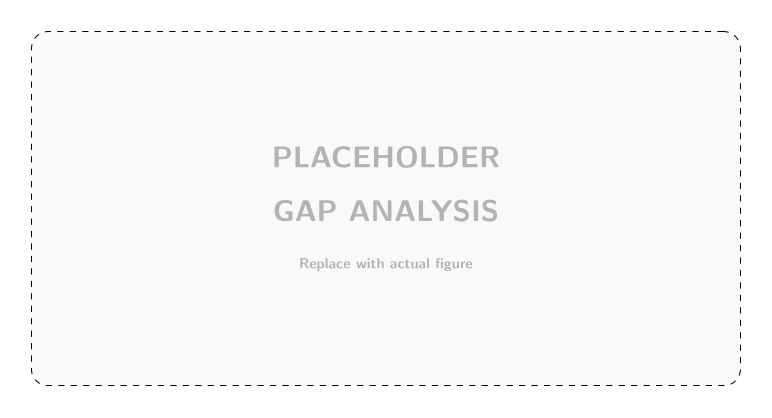
\includegraphics[width=0.85\textwidth]{Images/fig_gap_analysis.png}
\caption{Gap analysis showing unaddressed areas in existing e-voting literature that our system targets.}
\label{fig:gap-analysis}
\end{figure}

Our literature review reveals the following critical gaps:

\begin{enumerate}
    \item \textbf{Trusted Setup Elimination}: Most ZK voting systems (MACI, Semaphore) rely on Groth16, requiring a multi-party computation ceremony. No production voting system has deployed with a setup-free proof system like UltraHonk.
    
    \item \textbf{Gasless ZK Voting}: All existing blockchain voting systems either charge gas fees (excluding economically disadvantaged voters) or use centralized relayers. No system embeds the EVM in a sovereign chain with authority-sponsored execution.
    
    \item \textbf{Multi-Division National Architecture}: Academic prototypes model single-election contracts. Real national elections span hundreds of administrative divisions requiring on-chain aggregation, cross-division Sybil prevention, and delegated administration.
    
    \item \textbf{Mobile Hardware Security for Voting}: Voatz used biometrics but transmitted data to servers. No ZK voting system leverages device hardware keystores for voter secret storage with biometric gates and on-device proof generation.
    
    \item \textbf{Three-Factor Voter Authentication}: Existing systems use either wallet-only (weak) or centralized authentication. No system combines OTP, biometric, and hardware-backed cryptographic identity in a decentralized voting context.
    
    \item \textbf{Vote-Binding in ZK Proofs}: Standard Semaphore signals do not bind the signal content into the proof. This allows front-running attacks where a relayer observes the proof and substitutes a different vote. Our circuit binds the candidate index into the proof statement.
    
    \item \textbf{Administrative Hierarchy Modeling}: No prior work models the full government administrative hierarchy (Election Commission $\to$ District $\to$ Division $\to$ GN Division $\to$ Voter) with on-chain role delegation and access control.
\end{enumerate}

\section{Summary}

This literature review has surveyed the landscape from foundational cryptographic primitives through four generations of electronic voting systems. The key insight is that while individual building blocks exist---ZK proofs, blockchain consensus, mobile authentication, Merkle membership---no prior system integrates them into a cohesive, production-oriented architecture addressing real-world administrative requirements.

Our system (detailed in Chapters~\ref{ch:architecture}--\ref{ch:applications}) addresses each identified gap by combining UltraHonk proving (no trusted setup), a custom gasless blockchain (no economic barriers), multi-division factory contracts (administrative fidelity), and hardware-backed mobile authentication (three-factor security). The following chapter presents the system architecture that synthesizes these components into a unified design.
